\documentclass[12pt]{beamer}

    \usepackage[utf8]{inputenc}
    \usepackage{graphics}
    \usepackage{listings}
    
    \usepackage{array,booktabs}
    
    \usetheme{Madrid}
    \usecolortheme{beaver}
    
    % custom commands
    \newcommand{\nologo}{\setbeamertemplate{logo}{}} % set logo to empty
    
    \title{AMQP/Kafka/Kinesis}
    \author{Arun}
    \date{\today}
    
    \begin{document}
        \begin{frame}
            \begin{center}
                \frametitle{Message Queuing/Message Bus}
                \begin{itemize}
                    \item Message queuing allows applications to communicate by sending messages to each other. The message queue provides temporary message storage when the destination program is busy or not connected.
                \end{itemize}
            \end{center}
        \end{frame}
        
        \begin{frame}
            \begin{center}
                \frametitle{AMQP - Advanced Message Queuing Protocol}
                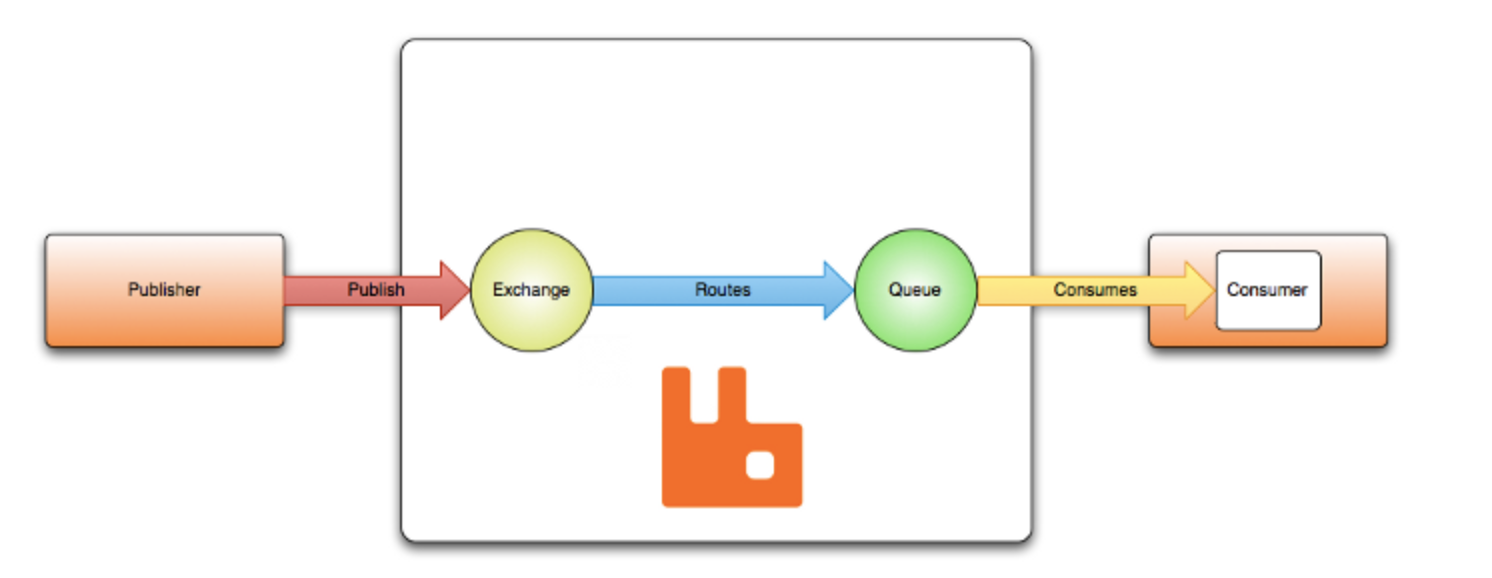
\includegraphics[width=0.5\textwidth]{images/simple-amqp}
                \begin{itemize}
                    \item AMQP 0.9.1 (latest version and what's supported by rabbitMQ)
                    \item publishers writes to the exchange, there are few routing options based on which the message is put in a queue
                    \item when a message cannot be routed, messages may be returned to publishers, dropped or put in dead letter queue
                    \item messages are stored until a consumer receives a message and acknowledge
                \end{itemize}
            \end{center}
        \end{frame}

        \begin{frame}
            \begin{columns}
                \column{0.4\textwidth}
                    \begin{center}
                        \frametitle{AMQP Direct Exchange}
                        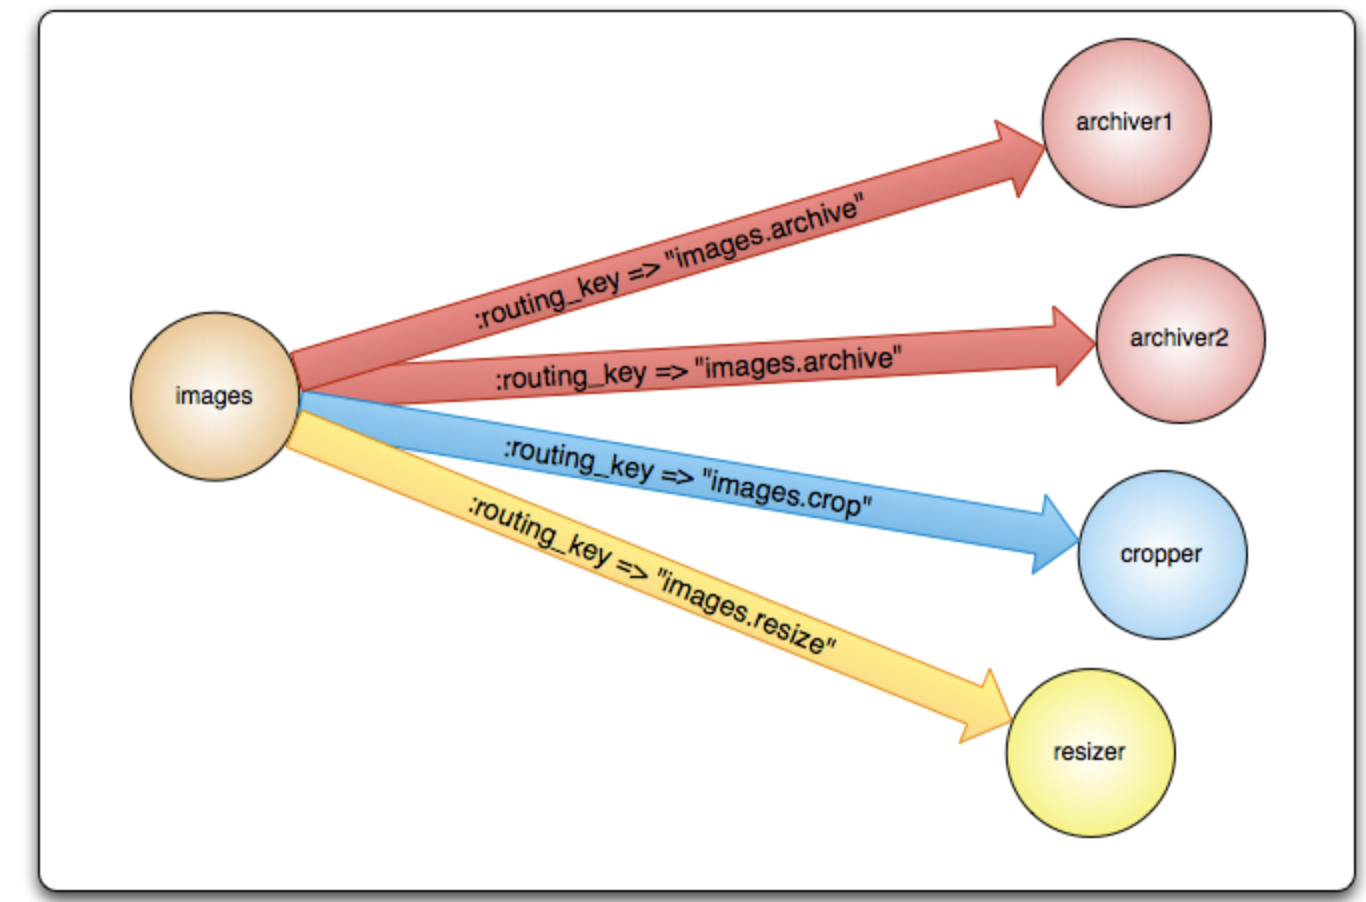
\includegraphics[width=1\textwidth]{images/direct-exchange}<1>
                        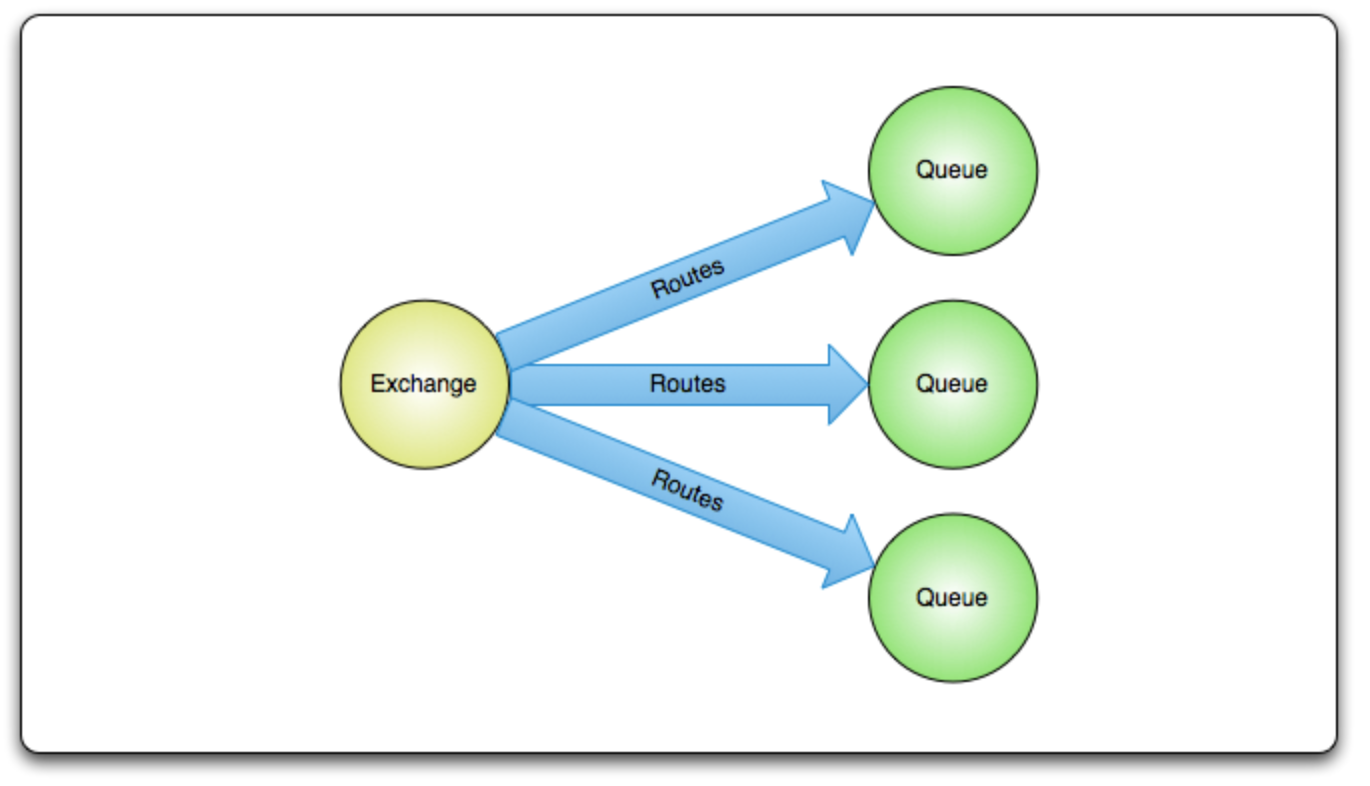
\includegraphics[width=1\textwidth]{images/fanout-exchange}<2>
                    \end{center}

                \column{0.6\textwidth}
                \begin{itemize}
                    \item Direct exchange (1-1 mapping)
                    \pause
                    \item Fanout exchange (1-n mapping)
                    \pause
                    \item Headers exchange ('x-match' header based), ...
                \end{itemize}
            \end{columns}
        \end{frame}

        \begin{frame}
            \begin{center}
                \frametitle{RabbitMQ scaling}
                \begin{itemize}
                    \item Consumer scaling is easy you can add more consumers when you publish quicker then you can consume
                    \item Scaling broker is veritcal in RabbitMQ.
                    \item Horizontal scaling of borker is possible with clustering but it's annowying setup
                \end{itemize}
            \end{center}
        \end{frame}

        \begin{frame}
            \begin{center}
                \frametitle{Kafka}
                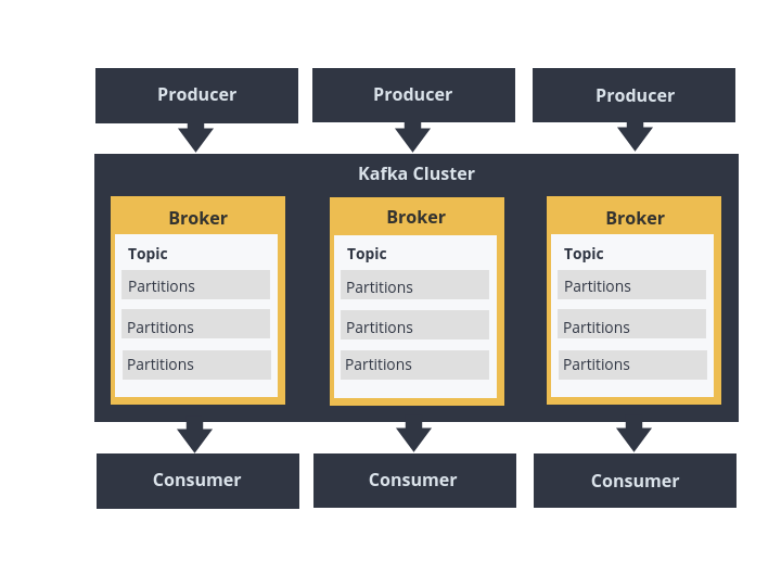
\includegraphics[width=0.5\textwidth]{images/kafka}
                \begin{itemize}
                    \item by LinkedIn, built for large scale stream processing in a fault-tolerant fashion with at-least once delivery
                    \item Kafka is based on the commit log, and messages comes from many producers in TCP
                    \item Data in a topic is partitioned and within a partition, messages are strictly ordered by their offsets
                    \item messages are stored until the set TTL is reached and can be replayed if needed with resetting the offsets
                    \item Kafka i bounded by IO and disk IOPS, and you can add more nodes/partition topics further to increase overcome those limits.
                \end{itemize}
            \end{center}
        \end{frame}

        \begin{frame}
            \begin{columns}
                    \column{0.4\textwidth}
                        \begin{center}
                            \frametitle{Kafka}
                            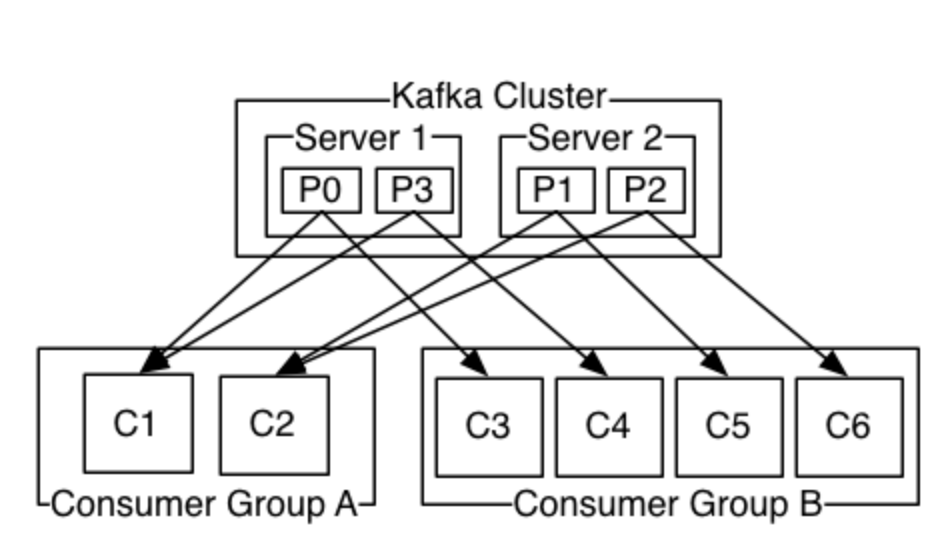
\includegraphics[width=1\textwidth]{images/kafka-consumer-groups}<2>
                            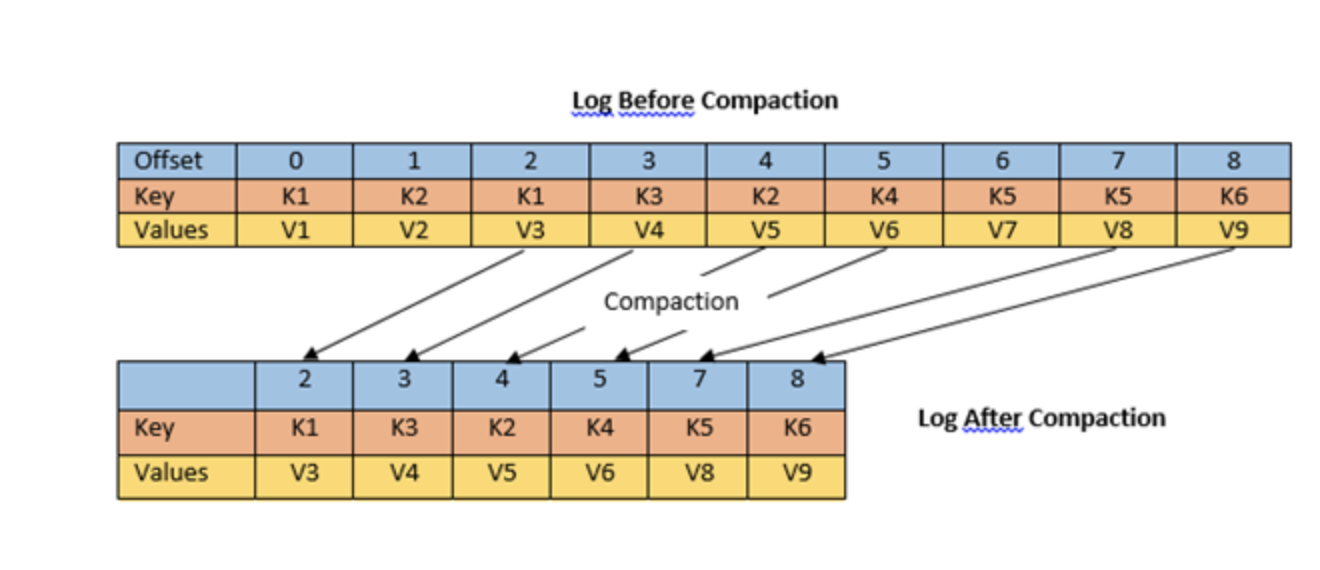
\includegraphics[width=1\textwidth]{images/kafka-compact-topics}<4>
                        \end{center}

                    \column{0.6\textwidth}
                        \begin{itemize}
                            \item 0.8.2 Most stable version of kafka, still with offsets stored in zookeeper
                            \pause
                            \item 0.9.x Consumer groups, offsets were stored in kafka itself as just another topic with immutable updates
                            \pause
                            \item 0.11 Kafka supports Exactly-once delivery using idempotent producer and transaction. 
                            \href{https://www.confluent.io/blog/exactly-once-semantics-are-possible-heres-how-apache-kafka-does-it/}{Blog}
                            \pause
                            \item 2.0 Compact topics - In simple terms, Apache Kafka will keep latest version of a record and delete the older versions with same key
                        \end{itemize}
            \end{columns}
        \end{frame}

        \begin{frame}
            \begin{center}
                \frametitle{Kafka and beyond}
                \begin{itemize}
                    \item Kafka now is a distributed streaming platform
                    \item Connect and Streams APIs
                    \item Mirroring (old but very powerful feature)
                \end{itemize}
            \end{center}
        \end{frame}
     
    \end{document}
    